This subsection presents the design of the deployment mechanism required to bring the inflatable from its stowed to its deployed configuration. It is key that this action is performed with maximum reliability, since deceleration of the entry vehicle and thereby mission success hinges on the aerodynamic surface area provided by the inflatable decelerator. This design comprises selection of a \acrfull{hdrm}, a canopy to protect the inflatable during interplanetary transfer and its detachment, and deployment.

Deployment of inflatables can be performed either by unrolling, unfolding or deploying a strut \cite[p.222-227]{Jenkins2001}. Figure \ref{fig:dep} serves as qualitative comparison between the principles of these systems. The unrolling and unfolding deployment mechanisms are deemed impractical for the following reason. Unrolling and unfolding in lateral direction from the centerbody are less package efficient than deploying it as a strut. Unrolling requires a hub about which is rolled and results in multiple toroids stacked together laterally. Unfolding compresses the toroids and thereby also features multiple toroids in lateral direction. Deploying, on the other hand, stretches the sphere cone shape in axial direction and thereby features less material in lateral direction. Unrolling and unfolding thus take up more space in radial direction through denser packing in this direction, while deploying stretches the packaging over the axial direction. 

A key driver for the use of inflatable aeroshells is the launch vehicle constraint on diameter in stowed configuration. By requiring less diameter for aeroshell package, more diameter is left free for the centerbody design. This results in maximum efficiency in the use of available diameter and thereby a more mass-efficient design, since an increase in centerbody diameter is deemed less mass-expensive than an increase in inflatable diameter for a given deployed diameter. This is a result supported by the sensitivity analysis presented in section \ref{subsec:strucsens}. 

\begin{figure}[h]
	\centering

	\begin{subfigure}[b]{0.49\textwidth}
		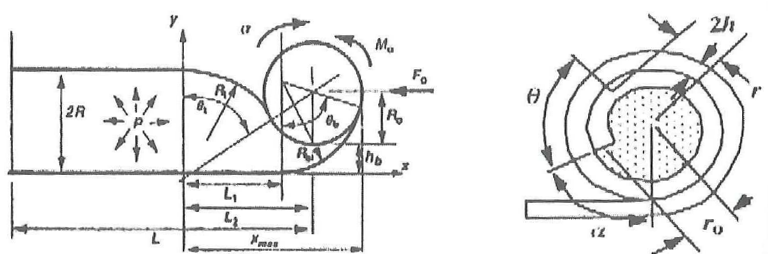
\includegraphics[width=0.96\textwidth]{./Figure/Structure/rot.png}
		\caption[Unrolling strut]{Unrolling strut \cite[p.222]{Jenkins2001}}
		\label{fig:rot}
	\end{subfigure}
	\begin{subfigure}[b]{0.49\textwidth}
		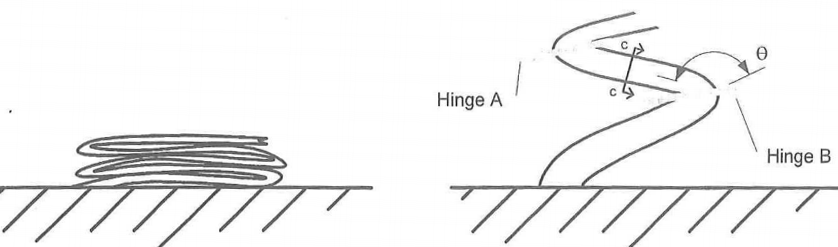
\includegraphics[width=0.96\textwidth]{./Figure/Structure/fold.png}
		\caption[Unfolding strut]{Unfolding strut \cite[p.226]{Jenkins2001}}
		\label{fig:fold}
	\end{subfigure}
		\begin{subfigure}[b]{1\textwidth}
		\centering
			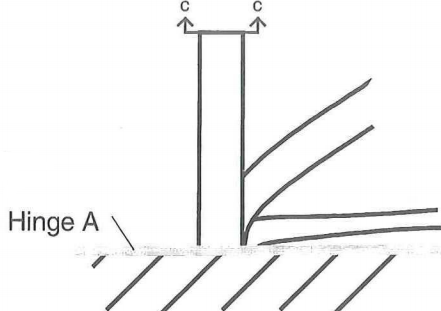
\includegraphics[width=0.3\textwidth]{./Figure/Structure/hinge.png}
			\caption[Deploying strut]{Deploying strut \cite[p.227]{Jenkins2001}}
			\label{fig:hinge}
		\end{subfigure}
	\caption[Overview of various deployment possibilities]{Overview of various deployment possibilities \cite{Jenkins2001}}
	\label{fig:dep}
\end{figure}


Moreover, less interference between flexible material is present when deploying the inflatable sphere cone as a hinge, as opposed to the folding and rolling of the toroids in the other two methods. This decreased amount of interference reduces the unpredictability and thereby increases reliability of the deployment procedure.

Deploying requires attachment points at which the outer toroid is held in place in stowed configuration. The axial length over which the inflatable is held in stowed condition is equal to the inflated radius minus the centerbody radius corrected for the half-cone angle, equal to XXX [m]. Attachment points will therefore be located at the side of the crew module, such that the inflatable is wrapped about the vehicle in stowed condition. 

The inflatable may moreover be covered by a shroud to provide additional protection from the space environment, primarily space debris, UV and radiation. A possible solution would be a coated Kevlar or Vectran canopy, as used for example in \gls{irve}-II \cite{Dillman2010}. For \gls{irve} the shroud weighed 1.9 [kg], for an approximate spanned area of 2 [$m^{2}$]. Upscaling this yields a shroud mass of 60 (CHECK ??) [$kg$] for the design at hand, where the shroud is required to span approximately 85 [$m^{2}$]. This shroud mass is significant on a decelerator mass of 1000 [$kg$] and such mass estimates are confirmed by a first-order estimate of a coated Vectran canopy, with a density of 1500 [$kg/m^{3}$] \cite{Miller2014}, which would yield a mass of 64 [$kg$] for half a millimeter thickness. Such a shroud is therefore unfeasible in terms of mass.

The canopy is not only unfeasible, but in addition not required. The outer layers of the inflatable are composed of Nextel, a material frequently applied as a micrometeoride shield\footnote{URL:\url{http://www.3m.com/market/industrial/ceramics/pdfs/outerspace_apps_brochure.pdf}. Accessed: 05-06-2015}. It is, as such, suitable for space application over prolonged periods of time, demonstrated by the \gls{iss} and ongoing research \cite{Thoma2005}, and provides sufficient protection against the space environment during interplanetary transfer. Moreover, the absence of a canopy relieves the issue of jettisoning it to prevent entanglement and aerodynamic interference after deployment and inflation.

The asymmetry of the inflatable does not form a problem, due to the foldability of the flexible material. The top of the inflatable is wrapped over itself such that the attachment ring is concentric with the crew module. 
%A shroud is wrapped about the inflatable to fulfill a twofold purpose: firstly to protect the inflatable from the space environment during interplanetary transfer, as they are susceptible to puncture, UV and radiation \cite{Cassapakis1995} and secondly to keep the inflatable in its stowed configuration. To this end the shroud should be durable within a space environment with sufficient stiffness for the transfer period. A lightweight solution would be a coated Kevlar or Vectran shroud. The restraint cover for the \gls{irve} vehicles weighed 1.9 [kg], for an approximate spanned area of 2 [m^{2}] \cite{Dillman2010}. Upscaling this yields a shroud mass of 60 (CHECK ??) [kg] for the design at hand. 

%REFERENCE
%aeroshell is another event of significant interest. Due to the high level of complexity associated with this event, the pre-flight strategy was to model deployment as a disturbance event. A wide range of disturbance torques were evaluated in the IRVE-II POST2 simulation to ensure the simulation had a high level of robustness in terms of the resulting entry performance, most importantly entry total angle of attack. In an attempt to put these disturbance torques into some context, a simulation was also conducted that emulated potential mass imbalance during the deployment. This mass imbalance was modeled after the evolution in shape of the aeroshell seen during full-scale deployment ground testing in the NASA Langley Research Center 16-m vacuum sphere. Images taken during this test can be seen in Figure 12. Since the vehicle is not spinning in the ground test it was unlikely this evolution would be duplicated in flight. However, it does provide some insight into bounding the problem. When simulating the mass properties of this shape evolution, the resulting tip-off rate equated to roughly a 12 N-m-s disturbance.
%In comparison to pre-flight analysis, the flight deployment occurred over a very short duration. As seen in the roll rate time history plotted in Figure 13. IRVE-II reaches its full roll inertia in less than 2 seconds. The effective tip-off rate of the deployment, seen in Figure 14, is 4.1 deg/sec. When cross-referenced with the pre-flight simulation this equates to a flight disturbance between 0 and 4 N·m·s.
%UP TO HERE
To prevent the inflatable from de-attaching from the centerbody and crew module during launch and transfer, a strap band is employed that wraps around the top of the inflatable and keeps it in place. The band features a cushioning part to prevent chafing and a bolt-and-nut clamping system that facilitates detachment. It is key that the strap band is reliable, both in terms of holding the inflatable to the centerbody and releasing it. An example product that fulfills these demands and has seen space application is produced by Voss Aerospace\footnote{URL:\url{http://vossind.com/assets/band-clamps---aerospace.pdf}. Accessed: 08-06-2015}. Pre-tensioning of the strap band and bolt-and-nut fastening mechanism are essential pre-flight activities to ascertain proper functioning.

To separate the bolt-and-nut fastening mechanism of the attachment belt and thereby initiate deployment events \glspl{hdrm} are used. As deployment is a singular event in time, one-time use is warranted. Reusable mechanisms typically have a larger number of moving parts and thereby a lower reliability than non-reusable mechanisms\footnote{URL:\url{http://www.esa.int/Our_Activities/Space_Engineering_Technology/Mechanisms/Hold-Down_and_Separation_Systems}. Accessed: 04-06-2015}. Reliability is key, since deployment of the aeroshell is of singular importance to aerodynamically decelerate the vehicle. To this end, pyrotechnic cutters are the pre-eminent solution by their high and proven reliability in space operations, low mass and low shock imparted to the vehicle. Example cutters are Chemring Hi-Shear cutters, applied in multiple space missions, such as the Mars observer mission\footnote{URL:\url{http://www.hstc.com/Products/OrdnanceProducts/CuttersBoltRodandCab/}. Accessed: 08-06-2015}. These possess a mass in the order of one hundred grams. For their criticality in mission success, redundancy of \glspl{hdrm} is key and multiple cutters are required to be present. 

This choice of separator mechanisms is moreover supported by an analysis for a tension cone, similar to a stacked toroid concept in deployment, by Miller et al. \cite{Miller2014}. Severing corset lacing by pyrotechnic cutters is therein deemed the most favourable option.

It is essential that the diameter of centerbody and crew module is slightly smaller than the maximum 5 [$m$] diameter to account for inflatable stowage. To this end, the centerbody diameter of XXX??? [$m$] rather than 5 [$m$] is imposed by deployment by taking into account a contingency of 5 $\%$.

Deployment is schematically summarized in Figure \ref{fig:deplflow}. Detachment is followed upon by inflation, which gives the inflated system the shape defined in subsection \ref{subsec:infldes}.

\begin{figure}[h]
		\centering
		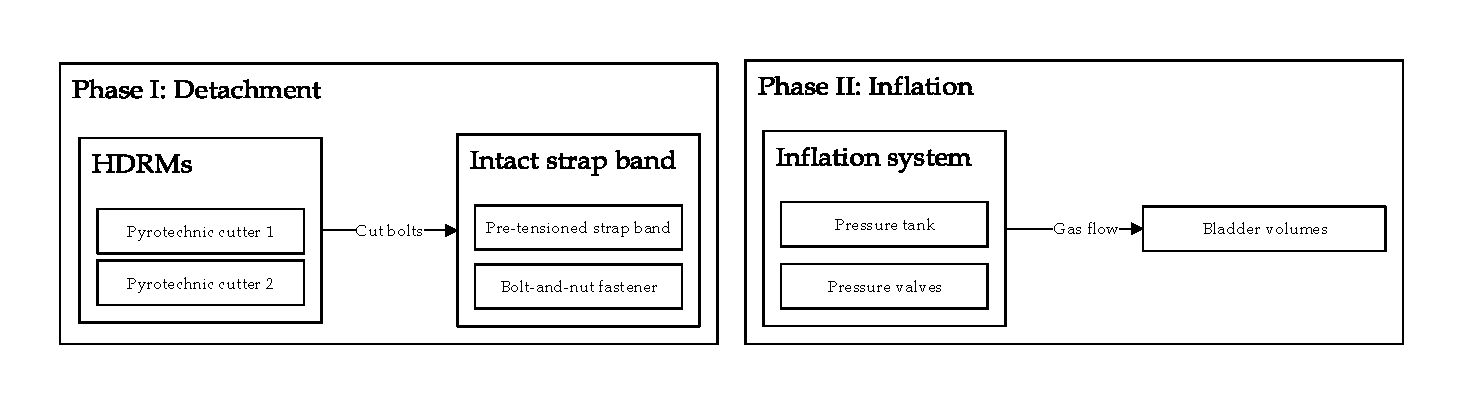
\includegraphics[width=1.0\textwidth]{./Figure/Structure/Deployment.pdf}
		\caption{Schematic view of deployment sequence}
		\label{fig:deplflow}
\end{figure}






